\textbf{Note:} You don't have to worry too much about how trees are actually represented as lists-- that's the power of abstraction at work!

As shown above, the tree constructor takes in a label and a list of branches (which are themselves trees).

\begin{lstlisting}

tree(4,
    [tree(5),
     tree(2,
        [tree(2),
         tree(1)]),
     tree(1),
     tree(8,
        [tree(4)])])
\end{lstlisting}

This creates a tree that looks like this:

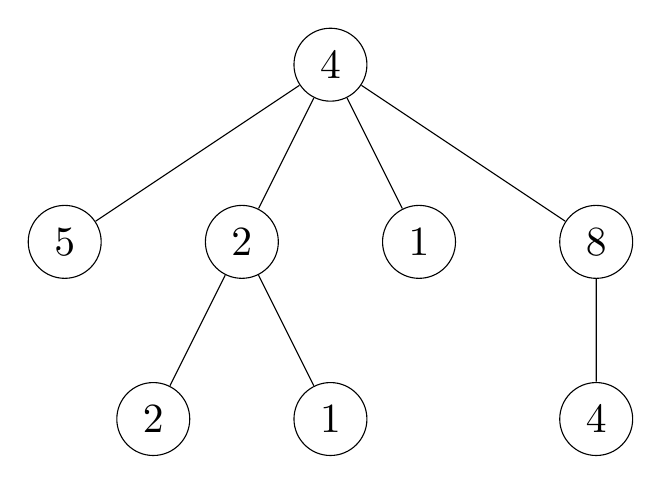
\begin{tikzpicture}[scale=1.5, transform shape]
    \node [circle, draw] (z){$4$}
        child {node [circle, draw] (a) {$5$}}
        child {node [circle, draw] (b) {$2$}
            child {node [circle, draw] (e) {$2$}}
            child {node [circle, draw] (f) {$1$}}
        }
        child {node [circle, draw] (c) {$1$}}
        child {node [circle, draw] (d) {$8$}
            child {node [circle, draw] (g) {$4$}}
        };
\end{tikzpicture}
% \end{blocksection}